\chapter{Related Studies }
In this chapter, principles and theories utilized in this thesis will be introduced.


% ------------------------------------------------------------ %
\section{Research Methodology}
In the methodology section, the we first delves into the existing literature, drawing from a paper accessible through the platform "Paper with Code." This platform typically provides research papers along with their associated code implementations. The chosen paper appears to be selected based on its prominence, likely measured by its reported accuracy or success in the field.
Following the identification of the primary paper, the researcher conducts a thorough review of its content, focusing particularly on aspects related to methodology. This involves understanding the proposed techniques, algorithms, and approaches presented in the paper to achieve high accuracy in the context of text-based person searches. The aim is to comprehend the nuances of the existing methodology and identify the key factors contributing to its success.
In addition to the primary paper, the researcher examines two other papers that exhibit a significant difference in accuracy. This comparative analysis is valuable for gaining insights into different approaches within the field. The choice of these additional papers may be strategic, aiming to capture diverse perspectives or methodologies, especially if there is a notable contrast in their reported accuracy metrics.
The researcher likely scrutinizes the methodologies of these selected papers, comparing and contrasting them with the primary paper. This comparative analysis helps identify the strengths and weaknesses of different approaches, shedding light on potential areas of improvement or innovation for the current research.
Overall, the methodology involves a comprehensive exploration of relevant literature, with a focus on the primary paper selected from "Paper with Code." The intent is to understand the methodologies employed in achieving high accuracies and to leverage insights from other papers with varying performance metrics. 

However, if only paperwithcode is used, the information obtained is limited and biased. To eliminate this bias, we decided to use scopus to search a wider range of papers by keyword search.

\subsection*{Identification}

The following research question was defined:

\bigskip
\textit{``How does the model compares with the text information with the image information''}
\bigskip



From this research question, four main keywords that sufficiently explain the topic were used: person retrieval and vision language pre-training.
Furthermore, synonyms and related terms were associated to these keywords to form keyword groups as follows:

\begin{itemize}
    \item person retrieval:
    \begin{itemize}
        \item person;
        \item person detection;
        \item person search.
    \end{itemize}
    \item vision language pre-training:
    \begin{itemize}
        \item VLP;
        \item text based;
        \item text.
    \end{itemize}
\end{itemize}


From the keywords, we had a keyword search on scopus from the search strings as follows:

\begin{itemize}
    \item ( "person retrieval" OR "person" OR "person detection" OR "person search" ) AND ( "vision language pre-training" OR "VLP" OR "text based" OR "text" ).
\end{itemize}

The Scopus search yielded a total of $20170$ documents. Within this result, we set the subject area to Computer Science, document type to article and conference paper, language to only english, and set the open access to all open access. With this filters, $862$ articles were found. 

\subsection{Screening}

Various factors were taken into account for the exclusion of documents:
\begin{enumerate}
    \item problem and goal were too different (e.g., building new hardware, analysis of leaf reflectance);
    \item not sufficiently related to this work (e.g., focused on hyperspectral );
    \item duplicates that were not automatically detected and excluded.
\end{enumerate}

% ------------------------------------------------------------ %

\section{Vision-language models}
Vision-language model have been researched significantly by leveraging end-to-end trainable deep neural networks (DNN). Before the vision-language model, both vision and language were researched with different DNN model structures. 

Vision recognition research have been updated until recent studies. Until now, the vision recognition models have experienced 5 stages, including traditional machine learning, deep learning from scratch, supervised pre-training with fine-tuning, unsupervised pre-training with fine-tuning, and vision-language model with pre-training.

Traditional machine learning relied on feature engineering. To achieve features, general methods were to hand-craft features \cite{svmclassification} and lightweight models \cite{knn}\cite{svm} to classify images into predefined categories. However, this method demands domain experts to design effective features for specific visual recognition tasks, which makes it ineffective for complex tasks and limits its scalability.

To overcome the problems with traditional methods, deep learning methods were devised \cite{imagenet} \cite{dnn_imagerecognition} to enhance the feature engineering and allowed to focus on the architecture engineering of neural networks to learn features effectively.
Great success from ResNet \cite{resnet}, which is a deep learning model introducing residual connections as a solution to the gradient vanishing problem. From this point, the deep learning demonstrated the ability to train on large datasets, achieving unprecedented performance. However, this approach faced issues such as slow training convergence and the need for extensive labeled data. 

Recent studies \cite{radford2021learning} have discovered that the features learned from large-scale labeled datasets possess a high degree of versatility and can be effectively transferred to a variety of downstream tasks. This indicates that the patterns and representations captured during the training on these extensive datasets are not only specific to the initial context but are also generalizable, allowing them to be utilized in different, often more specialized applications. This transferability underscores the potential of leveraging pre-trained models to enhance performance and efficiency in a wide range of tasks across various domains. 
This learning techniques accelerates training models with limited task-specific training datasets while achieving high performance.

The supervised pre-training outperformed many of the previous state-of-the-art performance on visual recognition tasks, yet still have the problem of preparing large-scale labeled datasets. To overcome the dependency on labeled data, Kaiming He, Haoqi Fan, et al.\cite{he2020momentumcontrastunsupervisedvisual} presented a method called Momentum Contrast (MoCo), which builds a dynamic dictionary with a queue and a moving-averaged encoder, enabling the model to learn effective representation without labeled data. Other methods are Simple Framework for Contrastive learning (SimCLR) introduced by Ting Chen, Simon Kornblith, et al. \cite{chen2020simpleframeworkcontrastivelearning}. This is a simplified contrastive learning framework for visual representation, avoiding specialized architectures or memory banks. 
Beyond this foundations, pre-training models no more rely on labeled datasets, which enabled to learn from various training data compared to supervised pre-training. 

For fine-tuning it requires labeled dataset for downstream tasks in both supervised or non-supervised pre-training models. Drastic improvements have emerged from natural language processing \cite{devlin2018bert}\cite{brown2020language}, combined with previous vision recognition, new paradigm called vision-language model (VLM) pre-training have proposed for vision recognition. To pre-train, this model does not requires to have labeled datasets, just requires image-text pairs. With this, the training datasets can be found infinitely in the internet. However, the image text pair in the internet contains information that does not correlate to each other. To train the model with some noise in the data, VLM is trained with certain vision-language objectives \cite{radford2021learning} \cite{yu2022cocacontrastivecaptionersimagetext}. From these objectives, the VLM 
matches the embedding of any given images and text, which enabled the performance of zero-shot prediction without fine-tuning on downstream visual recognition.

% Vision-Language models are a model that combines both the vision and language modalities and enables to process both information. 
% Take, for example, the task of zero-shot image classification. We’ll pass an image and a few prompts like so to obtain the most probable prompt for the input image.
% To predict the probable prompt, the model needs to understand both input image and the text prompts. To understand those modalities, the model will have separate or fused encoders for both vision and language.

\section{Model Used In This Thesis}
In this section, vision language model which is used in this thesis will be introduced.

\subsection{ALBEF}
Text encoder and image encoder are used to learn the representation in vision-and-language pre-training models (VLP). Most existing VLP models use multi-modal encoder to jointly model visual token (image feature) and word tokens (text features). This methods face challenges because the visual and word tokens are unaligned, making it difficult for the encoder to learn interactions between them. 
To tackle this challenge, the author first aligns image and text representations before fusing them through cross-modal attentions. 

\begin{figure}[htbp]
    \begin{center}
        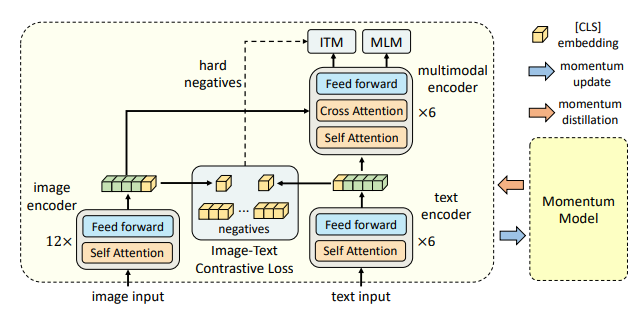
\includegraphics[width=\linewidth]{img/albef_model_structure.png}
        \caption{Structure of ALBEF}
        \label{fig:albef}
    \end{center}
\end{figure}

The author represented a model with an image encoder, text encoder, and a multi-modal encoder. They use 12-layer visual transformer ViT-B/16[\cite{dosovitskiy2021image}], pre-trained with ImageNet-1k, as the image encoder. 
Text encoder is pre-trained by the first 6 layers of $BERT_{base}$, and multi-modal encoder for fusing text and image features are pre-trained by the last 6 layers of $BERT_{base}$. The text encoder transform an input text $T$ into a sequence of embedding $\{w_{cls}, w_1, ..., w_N\}$. The image features also transform an input image $I$ into a sequence of embedding $\{v_{cls}, v_1, ..., v_M\}$. The text features are fed to a multi-modal encoder, while the image features are fused through cross attention at each layer of the multi-modal encoder.

Pretraining Objectives
The model have three objectives in pretraining: image-text contrastive learning (ITC) on the unimodal encoders, masked language modeling (MLM) and image-text matching (ITM).
Author utilizes the hard negative mined from ITC to improve ITM.

Image text contrastive learning is used to align the representation from the unimodal encoders before fusing. This objective makes it easier for the multi-modal encoder to perform cross-modal learning, as the input features are already aligned in a common space. 

Masked language modeling (MLM) is utilized with both image and text information to determine the masked text. Author randomly masks 15\% of the input token with specialized token [MASK]. The MLM minimizes the cross-entropy loss.

\begin{displaymath}
    L_{mlm} = \epsilon_{(I,\hat{T})~D}H(y^{msk}, p^{msk}(I,\hat{T}))
\end{displaymath}

$\hat{T}$ is masked text, $P^{msk}(I,\hat{T})$ is the model's predicted probability for a masked token. 

Contrastive loss is used for alignment, which helps to ground the vision and text representations.

\subsection{RaSa}

Vision language models are very popular regions. Many studies have been published to be able to bind the visual information with the text information. Many methods have been proposed, but learning a powerful multi-modal representation is still a challenging task. This author approaches to this task by two innovations: Relation aware and Sensitivity aware.

The author remarked that the text and image pair of the same ID have a strong positive pair and weak positive pair. Since the textual description is generated by a single image in the text-based person search dataset, the text will strongly correlate to the image but it is not always well-aligned to the other images of the same person. Previous methods did not take this intra-variation into account when training, they put the equal weight for strong and weak positive pairs in learning representations. This lead the model to overfitting due to the weak pairs.

To reduce the impact of noise interference from weak positive pairs, the author introduced a Relation-Aware learning (RA) task. This task consists of a probabilistic Image-Text Matching (p-ITM) component and a Positive Relation Detection (PRD) component. The p-ITM is a variant of the commonly used ITM, designed to differentiate negative and positive pairs by probabilistically considering strong or weak positive inputs. Meanwhile, the PRD explicitly distinguishes between strong and weak positive pairs. In this framework, p-ITM focuses on the consistency between strong and weak positive pairs, whereas PRD emphasizes their differences, effectively acting as a regularization for p-ITM. By incorporating RA, the model can extract valuable information from weak positive pairs through p-ITM and reduce noise interference through PRD, ultimately achieving a balance.

Furthermore, improving the robustness of representations often involves learning invariant representations under a set of manually chosen transformations, referred to as insensitive transformations [Caron et al., 2020; Chen and He, 2021]. While this approach is recognized, we take it further by drawing inspiration from the recent success of equivariant contrastive learning [Dangovski et al., 2022]. We explore sensitive transformations that would degrade performance if applied to learn transformation-invariant representations. Instead of maintaining invariance under insensitive transformations, we encourage the learned representations to be aware of sensitive transformations. 

To achieve this, author proposed a Sensitivity-Aware learning (SA) task. They use word replacement as the sensitive transformation and develop a Momentum-based Replaced Token Detection (m-RTD) pretext task. This task involves detecting whether a token originates from the original textual description or the replacement, as illustrated in Figure 1 (b). The closer the replaced word is to the original one (i.e., the more confusing the word), the more challenging the detection task becomes. Training the model to effectively solve this detection task is expected to enhance its ability to learn better representations.

The author utilize Masked Language Modeling (MLM) to perform word replacement, leveraging the image and text contextual tokens to predict the masked tokens. Additionally, considering that a momentum model, which is a slow-moving average of the online model, can learn more stable representations than the current online model [Grill et al., 2020], author use MLM from the momentum model to generate more confusing words. 

Overall, MLM and m-RTD together form Sensitivity-Aware learning (SA), providing robust surrogate supervision for representation learning.


\section{previous methods for masking strategies}


\section{Masking Strategies}
To extract finer features from the image and text inputs, 

Methods for masking have many different varieties, so from those methods, I pick to change the masking ratio.

\section{Visualize attention}
In this section, methology for visualization for attention towards the vision models. To understand how the vision model is recognizing the input images, many methods are introduced to describe the models perceptions.
\section{GradCAM}
Ramprasaath R. Selvaraju et al. presents a method for providing visual explanations for the decisions made by Convolutional Neural Networks (CNNs). This method, called Gradient-weighted Class Activation Mapping (Grad-CAM), generates a coarse localization map that highlights important regions in an image, which are crucial for predicting a specific concept.

Utilizes gradients flowing into the final convolutional layer to produce a localization map.
Applicable to various CNN architectures, including those with fully-connected layers (like VGG), models for structured outputs (like image captioning), and multi-modal inputs (like visual question answering).
Combining with Fine-Grained Visualizations:

Grad-CAM is combined with pixel-space gradient visualizations to create Guided Grad-CAM, which offers high-resolution, class-discriminative visualizations.
Applications and Insights:

Applied to image classification, image captioning, and visual question answering models.
Helps identify failure modes and dataset biases, providing insights into model predictions.
Demonstrates that even non-attention-based models can localize relevant input regions.
Human Studies:

Shows that Grad-CAM explanations help users build appropriate trust in model predictions.
Helps untrained users discern between stronger and weaker networks, even when their predictions are identical.
Benefits of Grad-CAM:

Does not require architectural changes or re-training of the network.
Outperforms previous methods in terms of weakly-supervised localization tasks and model faithfulness.
The paper emphasizes the importance of interpretability in AI systems, aiming to bridge the gap between model accuracy and transparency. By providing clear visual explanations, Grad-CAM enhances the trustworthiness and usability of deep learning models in practical applications.

\section{GradCAM++}
Aditya Chattopadhyay et al. introduces an enhanced version of the Grad-CAM method called Grad-CAM++. This method aims to provide better visual explanations of CNN model predictions by improving object localization and handling multiple object instances in a single image.

1. **Grad-CAM++ Method**:
   - Builds on Grad-CAM by introducing a generalized approach that uses a weighted combination of the positive partial derivatives of the last convolutional layer feature maps with respect to a specific class score to generate visual explanations.
   - Provides a mathematical derivation for the proposed method, making it computationally efficient and improving localization performance.

2. **Improvements Over Grad-CAM**:
   - Grad-CAM++ addresses limitations of Grad-CAM, such as difficulty in localizing multiple occurrences of the same class and partial object localization in single object images.
   - Introduces pixel-wise weighting of gradients to measure the importance of each pixel in a feature map towards the overall decision of the CNN.
   - Requires only a single backward pass on the computational graph, making it computationally equivalent to prior gradient-based methods while providing better visualizations.

3. **Evaluation and Metrics**:
   - Proposes new metrics to objectively evaluate the faithfulness of the visual explanations to the underlying model.
   - Demonstrates through experiments that Grad-CAM++ outperforms state-of-the-art methods in weakly supervised localization of object classes and other tasks like image captioning and 3D action recognition.

4. **Human Studies**:
   - Conducts human studies to assess the quality of the explanations produced by Grad-CAM++, showing that it instills greater trust in the underlying model compared to Grad-CAM.

5. **Applications**:
   - Effective in tasks beyond recognition, including image captioning and 3D action recognition.
   - Shows promising results in a teacher-student setting for knowledge distillation by using explanation maps generated by Grad-CAM++.

### Contributions:
- Grad-CAM++ provides a more general and accurate approach to visualizing CNN decisions.
- Improves trust in AI systems by providing clearer and more detailed explanations.
- Demonstrates applicability across various tasks and datasets, highlighting its robustness and versatility.

Overall, Grad-CAM++ represents a significant advancement in the field of explainable AI, particularly in improving the interpretability and transparency of deep learning models used in complex vision tasks.

\section{ScoreCAM}
Background
Understanding how convolutional neural networks (CNNs) make decisions is crucial for increasing their transparency and trustworthiness. Several methods have been developed for this purpose, including gradient-based methods, perturbation-based methods, and class activation mapping (CAM)-based methods.

Existing Methods
Gradient-Based Methods:

These methods highlight image regions that significantly influence the prediction by backpropagation the gradient of the target class to the input layer.
Examples include Saliency Maps and Grad-CAM. However, these methods often produce noisy and low-quality visual explanations.
Perturbation-Based Methods:

These involve perturbing the input image and observing changes in the model's predictions.
While these methods can be effective, they often require additional regularization and can be time-consuming.
CAM-Based Methods:

These create visual explanations by linearly combining activation maps from convolutional layers.
CAM is architecture-sensitive and requires a global pooling layer, which is not always present in all models.
Grad-CAM and Grad-CAM++ generalize CAM to work with models without a global pooling layer by using gradient information to weight the activation maps.
Score-CAM
The authors propose Score-CAM as a new method to address the limitations of existing gradient-based and CAM-based methods:

Gradient-Free: Unlike Grad-CAM, Score-CAM does not rely on gradient information, which can be noisy and prone to saturation issues.
Forward Passing Score: Score-CAM determines the weight of each activation map by its contribution to the target class score, assessed through a forward pass of the input.
Linear Combination: The final visual explanation is obtained by a linear combination of the weighted activation maps, which highlights the regions of the input image most relevant to the target class.
Methodology
Increase of Confidence: This concept quantifies the importance of each activation map by measuring the increase in the target class score when the corresponding activation map is used as input.
Implementation:
The method involves masking the input image with upsampled activation maps and measuring the change in the target score.
This change represents the importance of the activation map, which is then used as its weight.
Contributions and Evaluation
Fairness and Performance:

Score-CAM is evaluated on recognition tasks using metrics like Average Drop, Average Increase, Deletion curve, and Insertion curve, showing better evidence of the target class compared to other methods.
Qualitative evaluations also show better visualization and localization performance.
Debugging Tool:

The method is effective for analyzing and debugging model misbehaviors, providing insights into why a model made a specific prediction.

